\documentclass[emulatestandardclasses]{scrartcl}
\usepackage{graphicx}
\usepackage{color}
\usepackage[ngerman]{babel}
\usepackage{hyperref}
\usepackage{fullpage}
\usepackage{calc} 
\usepackage{enumitem}
\usepackage{titlesec}
\newcommand{\todo}[1]{\textcolor{red}{TODO: #1}\PackageWarning{TODO:}{#1!}}
\date{\vspace{-3ex}}
\begin{document}

\title{
	\includegraphics*[width=0.75\textwidth]{ErstesSem/images/hu_logo.png}\\
	\vspace{24pt}
	Hegels Ph"anomenologie des Geistes - ausgew"ahlte Kapitel}
\subtitle{Proseminar SS 17\\
          Dr. Dimitris Karydas\\
          Theologische Fakult"at \\ 
          Humboldt Universit"at zu Berlin}
\author{Lennard Wolf\\
        \small{\href{mailto:lennard.wolf@student.hu-berlin.de}{lennard.wolf@student.hu-berlin.de}}}
\maketitle
\begin{abstract}

Es werden Vorrede, Einleitung und ausgewählte Abschnitte des Werkes gelesen, die mit dessen Anliegen, systematischen Aufbau und der Durchführung einiger entscheidender argumentativer Züge vertraut machen sollten. Vorgesehen sind: die sinnliche Gewissheit, Bewusstsein und Selbstbewusstsein (Herrschaft und Knechtschaft), die absolute Freiheit und das absolute Wissen. Im close reading Verfahren sollte die systematisch geleitete Bewegung, in der der Unterschied des Bewusstseins überwunden wird, an ihren Knotenpunkten nachvollzogen werden.
\end{abstract}
\newpage

\tableofcontents
\listoffigures
\newpage


\section{Einf"uhrungssitzung\\(25.04.17)}

\subsection{Organisatorisches}

\begin{itemize}
  \item Moodle-PW: bewusst (ab 27.04.)
  \item Abgabe: Essay/Protokelle zu insgesamt 10 Seiten
  \item F"ur schein der Teilnahme ist ein Protokoll abzugeben
\end{itemize}

\subsection{Einf"uhrung}

\begin{itemize}
  \item Relevanz? Wird meist fetischistisch behandelt (sowohl positiv und negativ)
  \item Teil des kulturellen/gesellschaftlichen Ged"achtnisses
  \item Ohne Systematik macht Hegel keinen Sinn (Interpretation wird schwer/unm"oglich)
  \item Ziele der Veranstaltung: Fetischmismus soll abgebaut werden (mit Duktus/Systematik vertraut machen), Verst"andnis von Hegels Pr"agung/Relevanz f"ur unsere Zeit, Kontextualisierung des Werks innerhalb der Philosophie-Geschichte (Bez"uge herstellen zum Denken seiner Zeit, und heutigem Denken/Philosophieren)
  \item Einleitung ganz am Anfang geschrieben, Vorrede ganz am Ende
  \item 1806 begonnen, Fr"uhjahr 1807 erschienen, 7 Kapitel (gro"se Kapitel am Anfang, werden immer k"urzer wegen Zeitdruck (Fortbestehen der Uni Jena war unsicher wegen der nahenden Napoleonischen Truppen))
  \item Selbstbewusstsein als Leitfaden zur gesamten Struktur der P.d.G.
  \item S. d. B.s "`Das Zweite Geschlecht"' nach selber Struktur
  \item Bestandsaufnahme "uber die Erfahrung des Bewusstseins ("`Wissenschaft "uber die Erfahrung des Bewusstseins"')
  \item Hegel in einer lebenslangen Entwicklung - \emph{kein} fertiges System $\rightarrow$ kein gro"ses einheitliches System (!)
  \item Erstes gro"ses Buch Hegels (er hat nur wenige geschrieben)
  \item Arbeit am "`System"' ab 1802/03 in zweitem Drittel der Jenaer Zeit (3 Jenaer Systementw"urfe) $\rightarrow$ dadurch bekam er eine Vorstellung davon, was ein philosophisches System ist
  \item Zeit Hegels "`Zeit der gro"sen Systeme"', Beispiel: Festschrift der deutschen Philosophie
  \item Was ist ein System? \emph{Nicht}: Menge an Prinzipien, keine Gliederung von au"sen | \emph{Sondern}: Der Innere Zusammenhang des Ganzen, "`Das Wahre ist das Ganze"', Innere Orientierung am Ganzen, was die Welt am Innersten zusammenh"alt, "`einzige Darstellungsform des \emph{Wahren}"', Wahres nicht als Gegenteil vom Falschen, sondern das Wahre arbeitet aus dem Falschen heraus
  \item Adorno: "`Das Ganze ist das Unwahre"'
  \item Kants Philosophie ist die "`Folie"' auf der Hegel sich abarbeitet, Hauptbezugspunkt ($\rightarrow$ Buch selber zeigt sein kulturelles Ged"achtnis)
  \item Das \emph{Absolute} (Wissen) als Ergebnis des Buchs, "`Kristallnetz der Verkn"upfungen"' (Marx), "`Das Wesen des Denkens"' (\emph{nicht} wo alles gleich ist)
  \item "`Ph"anomenologie des Geistes"' als Einleitung zum System
  \item Philosophie der \emph{Idee}, dessen Tr"ager der Geist ist
  \item "`Realit"at"' ist das was ist, "`Wirklich"' sind die Strukturen dahinter
  \item "`Geist"': Kulturelle Produktion der Menschheitsgeschichte, die Selbstvorstellung des Menschen "uber sich
  \item Wissenschaft ist der Geist, der sich als Weist wei"s - Kulturelle Artefakte sind Versuche der Selbstvorstellung
  \item Junghegelianer, Linkshegelianer verstanden das Buch als Geschichtsphilosophie, Dozent: "uberzeugt von dem Argumenten \emph{dagegen}: 
  \item Buch war laut hegel erst zu dieser Zeit m"oglich (nicht 20 Jahre fr"uher), denn: Protestantismus und franz. Revolution sind Voraussetzung gewesen denn: Freiheit rechtlich kodifizeirt f"ur \emph{alle} $\rightarrow$ Geist thematisiert sich selbst, ohne "au"sere Einfl"usse, totale Selbstbez"uglichkeit
  \item Was nimmt sich das Buch vor? "`Unterschied des Bewusstseins"' "uberwinden (Unterschied zwischen Bildern, die sich das Bewusstsein von der Welt macht, und dem Gegenstand selbst)
  \item Erfahrungsgeschichte--?
  \item Alle Vorraussetzungen immer hinterfragen, "`Wo kommen die her?"'
\end{itemize}

"`\emph{Das Absolute? In unserer Welt?}"'


\section{Einleitung I, S. 53-62\\(02.05.17)}



\subsection{Lekt"urenotizen}

\begin{itemize}
  \item Betrachtung als Werkzeug? Dann ist es mittelbar und bringt nichts!
  \item Es ist nicht m"oglich, sich au"serhalb zu stellen!
  \item Wissen kann nicht begr"undet werden von innen. $\rightarrow$ Widerspruch!
  \item Darstellung des erscheinenden Wissens
  \item Einsicht in die Unwahrheit des erscheinenden Wissens
  \item Hegels Skeptizismus ist nicht als negativ aufzufassen, 
\end{itemize}

\subsection{Einleitung I, S. 53-62}

\begin{itemize}
  \item Einleitung steht vorher durch ihren Bezug zum Werk selber: \emph{Welcher Weg wird weshalb gegangen?}; Zwischen Polemik und Argumentation; Soll Leser in die Schuhe des AUtors stellen, dass das Ende schon bekannt ist!
  \item Vorrede kann auch parallel zum Gesamttext gelesen werden/auf diese kann sich immer
  \item Hegel grenzt sich ab von bisherigem Gedanken der Erkenntnistheorie, die einen Unterschied macht zwischen Methode der Erkenntnis und Erkanntem
  \item Er will "`nat"urliche Erkenntnis"' im Gegensatz zu Kant, der erst den theoretischen Gebrauch der Vernunft kl"aren wollte
  \item Wir \emph{sind} die Wahrnehmung - 
  \item Ziel: Undogmatische (Pr"amissenlose) Philosophie die zum Absoluten f"uhrt
  \item Was ist das Verh"altnis von wahrem und falschem ("`partikularem"') Wissen?
  \item Weg durch die Formen durch die \emph{bestimmte} (nicht abstrakte) Negation, welche keine Verneinung ist, sondern einen neuen Blickwinkel konstituiert durch "`Aufhebung"' des Negierten; 
  \item Nat"urliches Bewusstsein nur denkt Negation las vollst"andige Aufhebung und ist damit einseitig und primitiv
  \item Das Buch soll eine Philosophie der Freiheit begr"unden und stellt seine Einleitung dar (historisch)
  \item "`In der absoluten Idee steckt die absolute Methode"'
  \item Vollst"andigkeit der Form: Gew"ahrleistet durch die gezielte Negation
\end{itemize}

\begin{description}[leftmargin=!,labelwidth=\widthof{\bfseries Erscheinendes Bewusstsein}]
  \item[Die Wirklichkeit] Das was ist, vor der der Betrachtung. ("`Objekt"', muss aber auch als Subjekt gedacht werden!)
  \item[Die Realit"at] Die erscheinende Welt. (Das vom Subjekt wahrgenommene Objekt) |  Erscheinung/Ausdruck des Kreativen Geistes 
  \item[Das Absolute] Die Einheit von Subjekt und Objekt - Wesen und Erscheinung f"allt zusammen (nur im Geist m"oglich, durch den Vollzug der Weltgeschichte). \emph{oder} Struktur der Wirklichkeit (Die Vernunft, Struktur des Denkens). Es gibt nichts au"serhalb des Absoluten.
  \item[Absolutes Wissen] Regeln/Struktur des Denkens, nicht alles Wissen; Dem partikularen/realen Wissen wird immer weiter seine Partikularit"at genommen, bis Subjekt und Objekt ineinanderfallen
  \item[Reales Wissen] vom nat"urlichen Bewusstsein f"ur wirklich gehalten
  \item[Nat"urliche Erkenntnis] 
  \item[Erscheinendes Bewusstsein] 
  \item[Nat"urliches Bewusstsein] Einstellung, die Voraussetzungen eines bestimmten Verfahrens nicht hinterfragt | Jenes das sich als unmittelbar versteht | Dieses gilt es zu bek"ampfen
  \item[Geist] 
  \item[Form] 
  \item[Seele] Schnittstelle von Mensch und Tier
  \item[Ende der Geschichte] ?
  \item[Bestimmte Negation] Wenn man die konkreten Momente benennen kann, die negiert werden m"ussen: Ohne Ma"sstab von au"sen
\end{description}

Pluraletantum

\subsection{Der Aufbau der Phänomenologie des Geistes (Stephan Siemens)}

\begin{itemize}
  \item In einer dialektischen Philosophie, in der der Gedanke der Entwicklung bestimmend ist, verändern sich Inhalt und Form der Philosophie, damit aber auch das Verhältnis der Philosophie zu den Standpunkten, die die Philosophie von außen betrachten und von ihr äußerliche Rechtfertigungen verlangen.
  \item Die Hegelsche Philosophie verbindet das Denken der Totalität mit dem der Entwicklung (Dialketik)
\end{itemize}

\section{Einleitung II, S. 62-68\\(09.05.17)}

\subsection{Sitzung}

\begin{itemize}
  \item Wogegen grenzt sich Hegel ab? Das nat"urliche Bewusstsein/Verfahren
  \item Der Weg (die Bewegung) ist durch das Bewusstsein sein bestimmt
  \item Wissen ist die Seite des Gegenstandes des f"ur das Bewusstsein sein, das an sich ist die Wahrheit, das an sich ist auch f"ur es! 
  \item Ma"stab zur "Uberpr"ufung des gegenstands und sich selber wird vom Bewusstsein selbst gestellt; Bewusstsein seiner selbst
  \item Gegenstand (an sich) und Begriff (f"ur es) werden konstant gepr"uft! $\rightarrow$ Erfahrung
  \item Wissen: Was das Bewusstsein meint zu wissen... ("`Es ist 10 Uhr"')
  \item Wirklichkeit: Die tats"ahliche Uhrzeit.
  \item Wahrheit: bestimmte Negation das Wissen, ver"andert das WIssen, das Bewusstsein \emph{kann} das nicht merken, "`Wir"' schon
  \item logische Reduplikation
  \item "`Wir"' gucken dem Bewusstsein "uber die Schulter
  \item "`Wir"' wird mit dem Bewusstsein zusammenfallen, wenn "`es"' sich in "`unsere"' Position erhoben hat
  \item 1.: Das "`an sich f"ur es"', 2.: das "`an sich"', 3.: "`an sich f"ur uns"'
  \item Begriff: 
  \item "`Wir"': Auf dem STandpunkt des Ergebnisses des Buches; vollziehen die Erfahrung nach, das Bewusstsein "andert sich und damit das Bild (Wissen prallt auf Wahrheit), dabei "andert sich der Gegenstand, aber das Bewusstsein kann das nicht merken
  \item Das Bewusstsein verzweifelt weil es das Wissen updatet, der Gegenstand sich ver"andert, und das immer so weiter geht
  \item Wenn man denkt, man habe einen Begriff (in diesem Buch) verstanden, dann hat man ihn/es nicht verstanden.
\end{itemize}

\section{Sinnliche Gewi"sheit, S. 69-78\\(16.05.17)}

\subsection{Lekt"urenotizen}

\begin{itemize}
  \item Sinnliche Gewi"sheit: Erkenntnis deren konkreter Inhalt unendlich zu sein scheint, da er immer weiter teilbar ist 
  \item Sinnlichem Wissen ist das Wesentliche, dass die Sache \emph{ist}; Sinnliche Gewi"sheit ist unmittelbare Beziehung zwischen Einzelnem und Sache oder Bewu"stsein (Ich, reiner dieser)
  \item Das Allgemeine ist etwas das durch Negation ist; es ist das Wahre der sinnlichen Gewissheit -- WARUM?
  \item Wir \emph{meinen} das sinnliche Sein wenn wir sprechen, doch wir k"onnen immer nur das Allgemeine sagen
  \item Das Allgemeine ist nur durch einfaches Dieses vermittelbar
  \item Ist das Dies an sich allgemein?
  \item Vermittlung ist Negation
\end{itemize}

\begin{description}[leftmargin=!,labelwidth=\widthof{\bfseries Erscheinendes Bewusstsein}]
  \item[Reines Sein]
  \item[Allgemeines] Etwas das durch Negation ist; es ist das Wahre der sinnlichen Gewissheit
\end{description}

\subsection{Fragen}

\begin{itemize}
  \item Popper: reinforced dogmatism (https://de.wikipedia.org/wiki/Immunisierungsstrategie#Doppelt_verschanzter_Dogmatismus)
  \item Bereits Arthur Schopenhauer schrieb 1830, Dialektik sei die Kunst, in einem Disput immer Recht zu behalten.
  \item Ist nicht das partikulare Sein eines Gegenstands die Wahrheit der sinnlichen Gewissheit? was ist Wahrheit der sinnlichen Gewissheit? 
  \item ist nicht das allgemeine schon vermittelt? als allgemeines f"ur mich, wenn doch aber die sinnliche Gewissheit unmittelbar ist?
  \item Gibt es das Hier? Nein!
  \item Ist das Dies an sich allgemein?
\end{itemize}

Worum ging es in der Einleitung? Worum wird es gehen, wenn wir von Erfahrung des Bewusstseins sprechen? Was erf"ahrt das Bewusstsein? Worin besteht es? Wie kommt es zu Erfahrung? Prozess der Umkehrung/Selbstpr"ufung des Bewusstseins, sowie seines Bewusstseinsgegenstandes, wodurch das Bewusstsein etwas anderes wird. Und diese Ver"anderung ist die Erfahrung. So bestreitet es einen Weg, "uber welchen es zur Selbstthematisierung kommt. An sich: 


Wir können das Buch nur aus dem Standpunkt der heutigen Zeit lesen.



\newpage
\section{"Uber den Professor}
Prof. Mustermann ist..


%\begin{figure}[h]
%	\centering
%	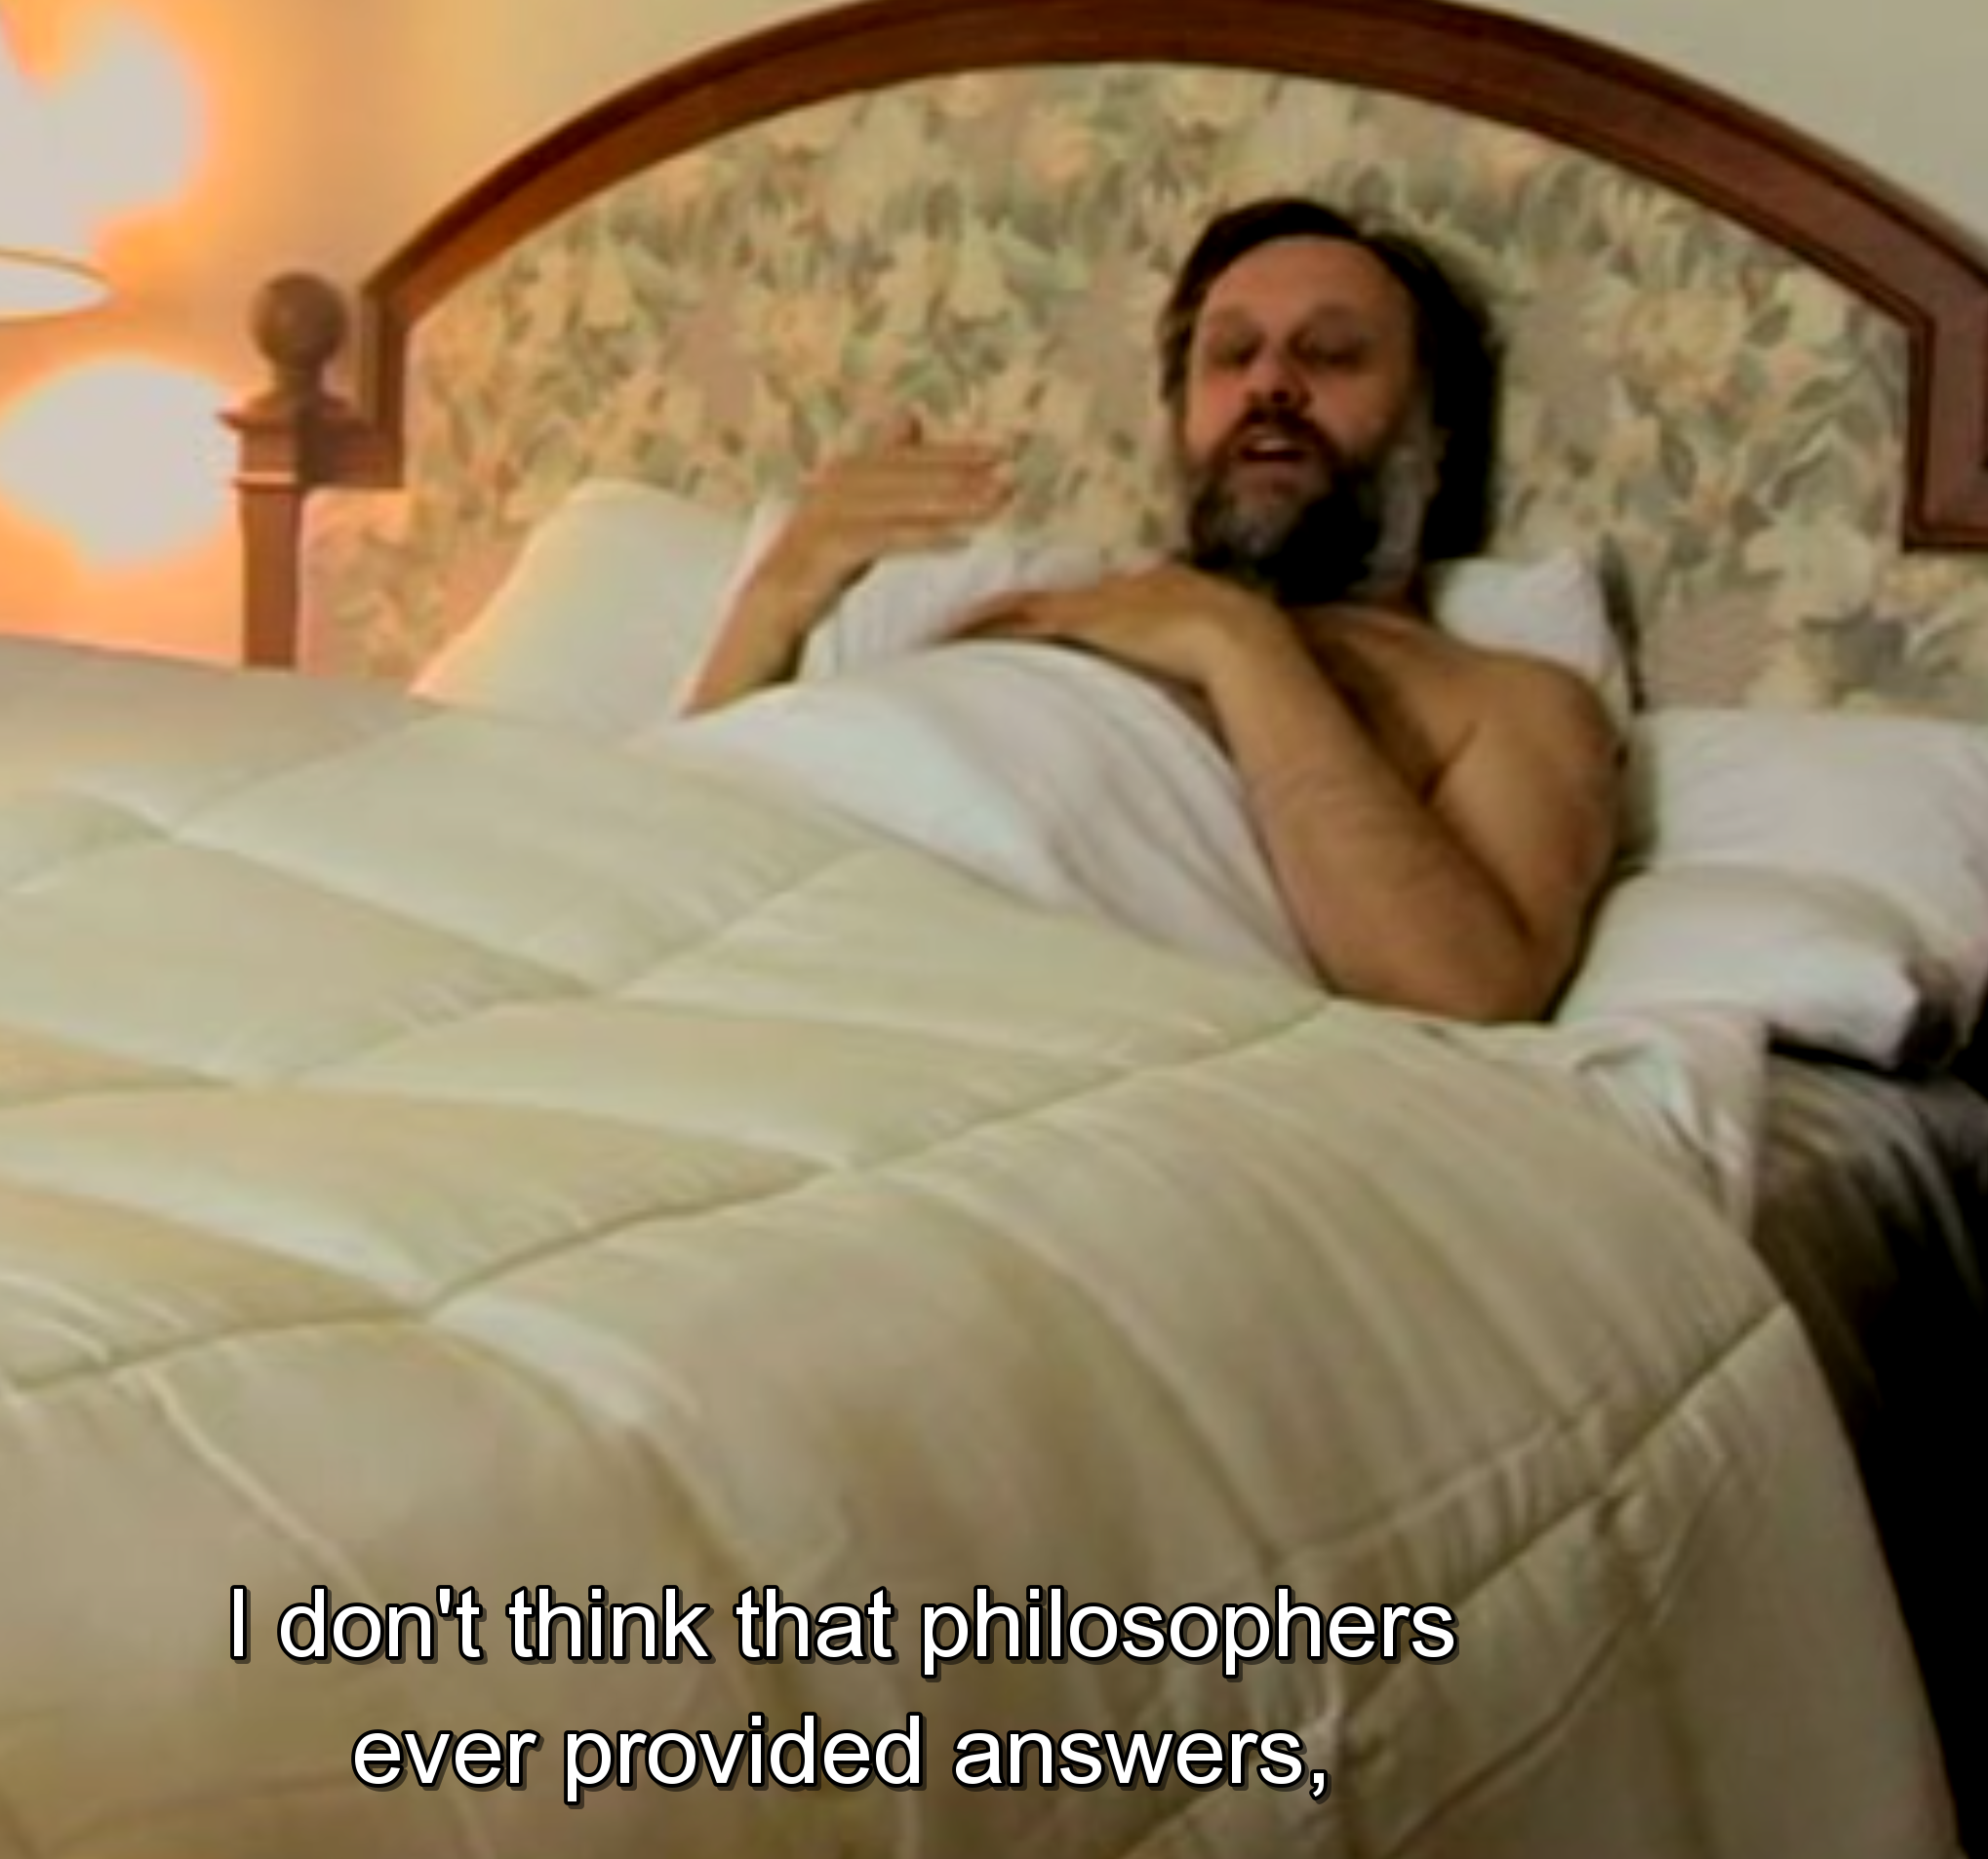
\includegraphics[width=0.5\textwidth]{images/template.png}
%	\caption{Template Bild}
%	\label{fig:template}
%\end{figure}

\end{document}
